\documentclass{BeamerTemplate}

\title{Chapitre 3 -- Estimations et tests d'hypothèse (3\textsuperscript{e} partie)}
\subtitle{STT-1920 Méthodes statistiques}
\date{}

% Styles des graphiques
\pgfplotsset{
  base/.style={
    tick label style={font=\scriptsize}, label style={font=\small},
    title style={font=\small\bfseries},
    yticklabel style={/pgf/number format/fixed, /pgf/number format/precision=2},
    scaled y ticks=false,
  },
  cloche/.style={
    base, axis lines=left, ytick=\empty, ymin=0,
    tick label style={font=\scriptsize},
  }
}

% Densités utilisées dans les figures
\def\dnorm{exp(-x^2/2)/sqrt(2*pi)}
% Student à 6 d.l. : constante Gamma(3,5)/(sqrt(6 pi) Gamma(3)) = 0,38273
\def\dtsix{0.38273*(1+x^2/6)^(-3.5)}

\begin{document}

\begin{frame}[t]
  \titlepage
\end{frame}

%===============================================================================
\section{Des hypothèses de recherche aux hypothèses statistiques}
%===============================================================================

\begin{frame}[t]{Où en sommes-nous?}
  \begin{itemize}\itemsep 2mm
    \item Au \alert{chapitre 3a}, nous avons \textbf{estimé} des paramètres ($\bar{x}$, $s^2$, $\hat{p}$) et mesuré leur précision (erreur-type).
    \item Au \alert{chapitre 3b}, nous avons construit des \textbf{intervalles de confiance}.
    \item<2-> Souvent, le chercheur doit plutôt \alert{prendre une décision} face à une affirmation :
      \begin{itemize}
        \item la concentration moyenne de mercure dépasse-t-elle la norme?
        \item la nouvelle diète augmente-t-elle la masse des souris?
      \end{itemize}
  \end{itemize}

  \vspace{-2mm}
  \uncover<3->{
  \begin{Boite}{Le test d'hypothèses}
    Une procédure qui permet de décider, à partir d'un échantillon, si les données fournissent une \alert{preuve suffisante} contre une affirmation. C'est l'outil de base des chapitres 4 à 7 (comparaisons de groupes, ANOVA, régression, khi-deux).
  \end{Boite}
  }
\end{frame}

\begin{frame}[t]{Des questions de recherche}
  Une question de recherche porte souvent sur un \alert{paramètre} d'une population :
  \begin{itemize}\itemsep 3mm
    \item<1-> \textbf{Toxicologie :} la concentration moyenne de mercure dans les dorés d'un réservoir est \alert{inférieure} à la ligne directrice de $0{,}5\ \mu$g/g.
    \item<2-> \textbf{Santé animale :} la prévalence d'une infection dans un troupeau \alert{dépasse} 10\%.
    \item<3-> \textbf{Pharmacologie :} l'écart-type de la dose de principe actif des comprimés est \alert{supérieur} à 2\,mg.
    \item<4-> \textbf{Physiologie :} la pression systolique moyenne d'une population \alert{diffère} de 130\,mm\,Hg.
  \end{itemize}

  \bigskip
  \uncover<5->{
    Chaque énoncé porte sur un paramètre ($\mu$, $p$, $\sigma$) et le compare à une \alert{valeur de référence}.
  }
\end{frame}

\begin{frame}[t]{Hypothèses statistiques : $H_0$ et $H_1$}
  \begin{Boite}{Hypothèse statistique}
    Énoncé sur la loi de probabilité d'une variable aléatoire, le plus souvent sur la valeur d'un paramètre (ex. : $\mu = 130$, $p > 0{,}10$, $\sigma^2 \ne 4$).
  \end{Boite}

  \vspace{-1mm}
  Un test confronte deux hypothèses, par exemple $H_0 : \mu = 25$ contre $H_1 : \mu > 25$.
  \begin{itemize}\itemsep 2mm
    \item<2-> $H_0$ : l'\alert{hypothèse nulle} (« rien de nouveau », « pas d'effet »). Elle est \alert{supposée vraie} tant que les données n'apportent pas une preuve suffisante du contraire.
    \item<3-> $H_1$ : l'\alert{hypothèse alternative}. Elle incarne l'effet ou le changement que le chercheur veut \alert{démontrer}.
  \end{itemize}
\end{frame}

\begin{frame}[t]{Quelques règles pour formuler $H_0$ et $H_1$}
  \begin{itemize}\itemsep 4mm
    \item $H_0$ et $H_1$ sont \alert{mutuellement exclusives}.
    \item $H_0$ contient toujours l'\alert{égalité} : $H_0 : \mu = \mu_0$, où $\mu_0$ est la valeur de référence.
    \item<2-> $H_1$ peut être :
      \begin{itemize}
        \item \alert{bilatérale} : $H_1 : \mu \ne \mu_0$ ;
        \item \alert{unilatérale} à droite ($H_1 : \mu > \mu_0$) ou à gauche ($H_1 : \mu < \mu_0$).
      \end{itemize}
    \item<3-> C'est l'\alert{hypothèse de recherche} (ce qu'on veut démontrer) qui dicte $H_1$, et elle doit être fixée \alert{avant} de voir les données.
  \end{itemize}
\end{frame}

\begin{frame}[plain,t]
  \centerline{\LARGE\bfseries\alert{QUIZ !}}

  \medskip
  Formulez $H_0$ et $H_1$ :
  \begin{itemize}\itemsep 0.9cm
    \item Un agronome veut démontrer qu'un nouvel engrais porte le rendement moyen du blé \alert{au-delà} de 3,5\,t/ha.
    \item<2-> Une biologiste veut vérifier si la proportion de tiques porteuses de la bactérie de Lyme dans un parc \alert{dépasse} 20\%.
    \item<3-> Un médicament \alert{modifie}-t-il la fréquence cardiaque moyenne au repos (72 battements/min)?
    \item<4-> Sur 10 parcelles fertilisées, l'agronome obtient $\bar{x} = 3{,}62$\,t/ha. Peut-il conclure que l'engrais est efficace?
  \end{itemize}
\end{frame}

%===============================================================================
\section{La logique d'un test}
%===============================================================================

\begin{frame}[t]{Exemple 7 : une diète enrichie chez la souris}
  Dans une lignée de souris de laboratoire, la masse à 8 semaines suit une loi $\mathcal{N}(\mu,\ \sigma^2 = 2^2)$ ; sous la diète standard, $\mu = 25$\,g.
  Grâce aux nombreuses données historiques, on considère $\sigma = 2$\,g comme \alert{connu}.

  \medskip
  On nourrit $n = 16$ souris avec une \alert{diète enrichie} et on obtient $\bar{x} = 26{,}1$\,g.

  \medskip
  \uncover<2->{
    \textbf{Question :} la diète enrichie augmente-t-elle la masse moyenne? (seuil $\alpha = 5\%$)
  }

  \medskip
  \uncover<3->{
    $$H_0 : \mu = 25 \qquad \text{contre} \qquad H_1 : \mu > 25$$
  }

  \uncover<4->{
    \textbf{Le dilemme :} $26{,}1 > 25$, mais $\overline{X}$ varie d'un échantillon à l'autre. L'écart de $1{,}1$\,g est-il \alert{trop grand pour être dû au hasard} si $H_0$ est vraie?
  }
\end{frame}

\begin{frame}[t]{Les étapes d'un test d'hypothèses}
  \begin{enumerate}\itemsep 1.5mm
    \item<1-> \textbf{Hypothèses :} formuler $H_0$ et $H_1$ et choisir le \alert{seuil} $\alpha$.
    \item<2-> \textbf{Statistique de test :} choisir une statistique dont on connaît la \alert{loi si $H_0$ est vraie}.
    \item<3-> \textbf{Règle de décision :} déterminer la \alert{région de rejet} (ou utiliser la valeur-p).
    \item<4-> \textbf{Calcul :} calculer la statistique observée à partir de l'échantillon.
    \item<5-> \textbf{Décision et conclusion :} rejeter ou ne pas rejeter $H_0$, puis conclure \alert{dans les termes de l'étude}.
  \end{enumerate}

  \uncover<6->{
  \begin{Boite}{Seulement deux décisions possibles}
    « On rejette $H_0$ » ou « on ne rejette pas $H_0$ ». On ne dit jamais « on accepte $H_0$ ».
  \end{Boite}
  }
\end{frame}

\begin{frame}[t]{Statistique de test et loi sous $H_0$}
  Si $H_0$ est vraie ($\mu = \mu_0$), alors $\overline{X} \sim \mathcal{N}(\mu_0, \sigma^2/n)$ et on standardise :
  $$Z_0 = \frac{\overline{X} - \mu_0}{\sigma/\sqrt{n}} \sim \mathcal{N}(0,1) \quad \text{sous } H_0.$$

  \vspace{-2mm}
  \begin{columns}[T]
    \column{0.49\textwidth}
      \centering
      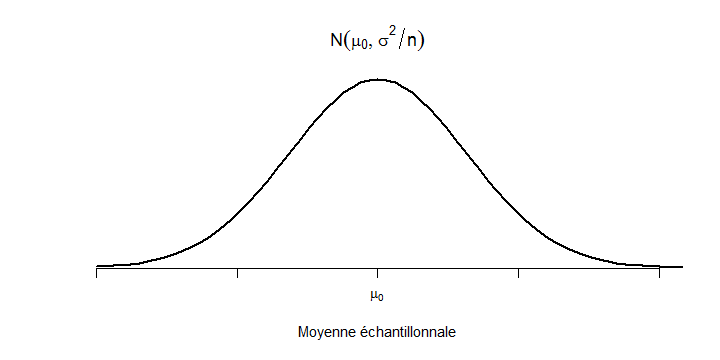
\includegraphics[width=\linewidth]{images/H0-xbarre-gen.png}

      {\scriptsize Loi de $\overline{X}$ sous $H_0$}
    \column{0.49\textwidth}
      \centering
      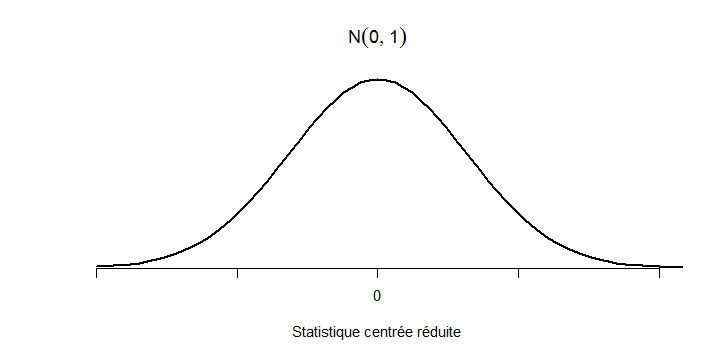
\includegraphics[width=\linewidth]{images/H0-z.png}

      {\scriptsize Loi de $Z_0$ sous $H_0$}
  \end{columns}

  \medskip
  \uncover<2->{
    Exemple 7 : $z_{obs} = \dfrac{26{,}1 - 25}{2/\sqrt{16}} = \dfrac{1{,}1}{0{,}5} = \mathbf{2{,}2}$ : la moyenne observée est à 2,2 erreurs-types de $\mu_0$.
  }
\end{frame}

\begin{frame}[t]{Règle de décision et région de rejet}
  On rejette $H_0 : \mu = 25$ en faveur de $H_1 : \mu > 25$ si $\bar{x}$ est \alert{trop grand}, c'est-à-dire si $z_{obs}$ tombe dans les $\alpha = 5\%$ les plus extrêmes \alert{à droite} de la loi $\mathcal{N}(0,1)$.

  \centering
  \begin{tikzpicture}
    \begin{axis}[cloche, width=10cm, height=4.2cm, xmin=-3.5, xmax=4.5, ymax=0.45,
      xtick={0,1.645}, xticklabels={0, $z_{0{,}05} = 1{,}645$}]
      \addplot[draw=none, fill=Accent!70, domain=1.645:4.5, samples=40] {\dnorm} \closedcycle;
      \addplot[thick, Dominante!70!black, domain=-3.5:4.5, samples=120] {\dnorm};
      \node[font=\scriptsize] at (axis cs:0,0.15) {Non-rejet de $H_0$};
      \node[font=\scriptsize, Accent!80!black, align=center] at (axis cs:3.6,0.2) {Région de rejet\\ aire $\alpha = 0{,}05$};
      \draw[->, Accent!80!black] (axis cs:3.5,0.15) -- (axis cs:2.6,0.02);
      \uncover<2->{\draw[very thick, rougelaval] (axis cs:2.2,0) -- (axis cs:2.2,0.30);
      \node[rougelaval, font=\scriptsize, left] at (axis cs:2.2,0.30) {$z_{obs} = 2{,}2$};}
    \end{axis}
  \end{tikzpicture}

  \raggedright
  \textbf{Règle :} rejeter $H_0$ si $z_{obs} > z_{\alpha} = 1{,}645$.
  \quad Sur l'échelle de $\bar{x}$ : si $\bar{x} > 25 + 1{,}645 \times 0{,}5 = 25{,}82$\,g.
\end{frame}

\begin{frame}[t]{Exemple 7 (suite) : décision et conclusion}
  \begin{enumerate}\itemsep 3mm
    \item \textbf{Hypothèses :} $H_0 : \mu = 25$ contre $H_1 : \mu > 25$, avec $\alpha = 0{,}05$.
    \item \textbf{Statistique :} $Z_0 = \frac{\overline{X} - 25}{2/\sqrt{16}} \sim \mathcal{N}(0,1)$ sous $H_0$.
    \item \textbf{Règle de décision :} rejeter $H_0$ si $z_{obs} > 1{,}645$.
    \item<2-> \textbf{Calcul :} $z_{obs} = 2{,}2$.
    \item<3-> \textbf{Décision :} $2{,}2 > 1{,}645$, donc on \alert{rejette $H_0$}.
  \end{enumerate}

  \uncover<4->{
  \begin{Boite}{Conclusion dans les termes de l'étude}
    Au seuil de 5\%, les données démontrent que la diète enrichie \alert{augmente} la masse moyenne des souris de 8 semaines.
  \end{Boite}
  }
\end{frame}

%===============================================================================
\section{Erreurs de type I et II}
%===============================================================================

\begin{frame}[t]{Deux erreurs possibles}
  La décision est prise à partir d'un échantillon : on peut se tromper !

  \medskip
  \centering
  \renewcommand{\arraystretch}{1.5}
  \begin{tabular}{l|cc}
    & \multicolumn{2}{c}{\textbf{Réalité (inconnue !)}} \\
    \textbf{Décision} & $H_0$ vraie & $H_0$ fausse \\ \hline
    Rejeter $H_0$ & \alert{Erreur de type I} & Bonne décision \\
    Ne pas rejeter $H_0$ & Bonne décision & \alert{Erreur de type II} \\
  \end{tabular}

  \raggedright
  \medskip
  \uncover<2->{
  \begin{itemize}\itemsep 2mm
    \item $\alpha = P(\text{erreur de type I}) = P(\text{rejeter } H_0 \mid H_0 \text{ vraie})$ : le \alert{seuil} du test.
    \item $\beta = P(\text{erreur de type II}) = P(\text{ne pas rejeter } H_0 \mid H_0 \text{ fausse})$.
    \item $1 - \beta = P(\text{rejeter } H_0 \mid H_0 \text{ fausse})$ : la \alert{puissance} du test.
  \end{itemize}
  }
\end{frame}

\begin{frame}[t]{Deux analogies}
  \vspace{-3mm}
  \begin{columns}[T]
    \column{0.48\textwidth}
      \begin{Boite}{\faBalanceScale\ Un procès}
        \small
        \begin{itemize}\itemsep 1mm
          \item $H_0$ : l'accusé est innocent ; $H_1$ : il est coupable.
          \item On condamne seulement si la preuve est \alert{hors de tout doute raisonnable}.
          \item Type I : condamner un innocent. Type II : acquitter un coupable.
          \item Acquitter $\ne$ prouver l'innocence !
        \end{itemize}
      \end{Boite}

    \column{0.48\textwidth}
      \uncover<2->{
      \begin{Boite}{\faStethoscope\ Un test diagnostique}
        \small
        \begin{itemize}\itemsep 1mm
          \item $H_0$ : le patient n'a pas la maladie ; $H_1$ : il l'a.
          \item Type I : \alert{faux positif}. Type II : \alert{faux négatif}.
          \item $1 - \alpha$ correspond à la \alert{spécificité}, la puissance $1 - \beta$ à la \alert{sensibilité}.
        \end{itemize}
      \end{Boite}
      }
  \end{columns}
\end{frame}

\begin{frame}[t]{Visualiser $\alpha$ et $\beta$ (exemple 7)}
  \small
  Si en réalité la diète fait passer la moyenne à $\mu_1 = 26$\,g, $\overline{X} \sim \mathcal{N}(26,\ 0{,}5^2)$ au lieu de $\mathcal{N}(25,\ 0{,}5^2)$.

  \centering
  \begin{tikzpicture}
    \begin{axis}[cloche, width=11cm, height=4.6cm, xmin=23.3, xmax=27.7, ymax=0.95,
      xtick={25,25.82,26}, xticklabels={$\mu_0 = 25$, , $\mu_1 = 26$}, xlabel={$\bar{x}$ (g)}]
      \addplot[draw=none, fill=Dominante!45, domain=23.3:25.822, samples=60] {exp(-(x-26)^2/(2*0.25))/(0.5*sqrt(2*pi))} \closedcycle;
      \addplot[draw=none, fill=Accent!75, domain=25.822:27.7, samples=60] {exp(-(x-25)^2/(2*0.25))/(0.5*sqrt(2*pi))} \closedcycle;
      \addplot[thick, black, domain=23.3:27.7, samples=120] {exp(-(x-25)^2/(2*0.25))/(0.5*sqrt(2*pi))};
      \addplot[thick, black, dashed, domain=23.3:27.7, samples=120] {exp(-(x-26)^2/(2*0.25))/(0.5*sqrt(2*pi))};
      \draw[rougelaval, thick] (axis cs:25.822,0) -- (axis cs:25.822,0.9);
      \node[rougelaval, font=\scriptsize, right] at (axis cs:25.822,0.88) {seuil de rejet : $25{,}82$};
      \node[font=\scriptsize] at (axis cs:24.1,0.6) {Sous $H_0$};
      \node[font=\scriptsize] at (axis cs:27.0,0.6) {Sous $H_1$ ($\mu = 26$)};
      \node[font=\small\bfseries, Dominante!40!black] at (axis cs:25.5,0.1) {$\beta$};
      \node[font=\small\bfseries, Accent!40!black] at (axis cs:26.02,0.035) {$\alpha$};
    \end{axis}
  \end{tikzpicture}

  \raggedright
  \uncover<2->{
    $\alpha = 0{,}05$ (orange) ; \ $\beta = P(\overline{X} \le 25{,}82 \mid \mu = 26) = 0{,}361$ (bleu) ; \ puissance $= 1 - \beta = \mathbf{0{,}639}$.
  }
\end{frame}

\begin{frame}[t]{Quelques remarques importantes}
  \begin{itemize}\itemsep 4mm
    \item L'erreur de type I est habituellement jugée la plus grave : on fixe $\alpha$ \alert{petit} ($0{,}05$ ou $0{,}01$) \alert{avant} l'analyse.
    \item<2-> À $n$ fixe, diminuer $\alpha$ \alert{augmente} $\beta$ (la ligne rouge se déplace vers la droite).
    \item<3-> On contrôle donc $\alpha$ directement, et $\beta$ surtout par la \alert{taille d'échantillon}.
    \item<4-> $\beta$ est souvent grand avec de petits échantillons : « ne pas rejeter $H_0$ » signifie seulement que la preuve est \alert{insuffisante}, pas que $H_0$ est vraie.
  \end{itemize}

  \bigskip
  \uncover<5->{
  \begin{Boite}{L'absence de preuve n'est pas la preuve de l'absence}
    Un test non significatif ne démontre pas l'absence d'effet.
  \end{Boite}
  }
\end{frame}

\begin{frame}[plain,t]
  \centerline{\LARGE\bfseries\alert{QUIZ !}}

  \medskip
  \begin{itemize}\itemsep 1.2cm
    \item Dans l'exemple 7, décrivez en mots une erreur de type I et une erreur de type II.
    \item<2-> On dépiste une maladie grave mais traitable ($H_0$ : patient sain). Quelle erreur est la plus grave? Que faut-il privilégier?
    \item<3-> Vrai ou faux : si on ne rejette pas $H_0$, la probabilité que $H_0$ soit vraie est $1 - \alpha$.
  \end{itemize}
\end{frame}

%===============================================================================
\section{La valeur-p}
%===============================================================================

\begin{frame}[t]{La valeur-p (seuil observé)}
  \begin{Boite}{Valeur-p}
    \small
    Probabilité, \alert{si $H_0$ est vraie}, d'obtenir une statistique de test \alert{au moins aussi extrême} (dans le sens de $H_1$) que celle observée.
    C'est aussi le plus petit $\alpha$ pour lequel on rejetterait $H_0$ avec ces données.
  \end{Boite}

  \begin{columns}[T]
    \column{0.52\textwidth}
      \begin{tikzpicture}
        \begin{axis}[cloche, width=6.8cm, height=3.5cm, xmin=-3.5, xmax=3.5, ymax=0.45,
          xtick={0,2.2}, xticklabels={0, $2{,}2$}]
          \addplot[draw=none, fill=Accent!75, domain=2.2:3.5, samples=30] {\dnorm} \closedcycle;
          \addplot[thick, Dominante!70!black, domain=-3.5:3.5, samples=100] {\dnorm};
          \node[font=\scriptsize, Accent!80!black] at (axis cs:2.6,0.17) {$0{,}0139$};
          \draw[->, Accent!80!black] (axis cs:2.6,0.14) -- (axis cs:2.45,0.02);
        \end{axis}
      \end{tikzpicture}

    \column{0.46\textwidth}
      \small
      \textbf{Exemple 7 :}
      valeur-p $= P(Z \ge 2{,}2) = 0{,}0139$.

      \medskip
      \uncover<2->{
      \begin{Boite}{Règle universelle}
        Rejeter $H_0$ au seuil $\alpha$ $\iff$ valeur-p $\le \alpha$.
      \end{Boite}
      Ici $0{,}0139 \le 0{,}05$ : on rejette $H_0$.
      }
  \end{columns}
\end{frame}

\begin{frame}[t]{Calcul de la valeur-p selon $H_1$}
  Soit $z_{obs}$ la valeur observée de $Z_0$ (même principe pour $t_{obs}$ avec la loi $t_{n-1}$) :

  \medskip
  \centering
  \renewcommand{\arraystretch}{1.6}
  \begin{tabular}{lll}\toprule
    \textbf{Alternative} & \textbf{Valeur-p} & \textbf{Rejet de $H_0$ au seuil $\alpha$ si} \\ \midrule
    $H_1 : \mu > \mu_0$ (droite) & $P(Z \ge z_{obs})$ & $z_{obs} > z_{\alpha}$ \\
    $H_1 : \mu < \mu_0$ (gauche) & $P(Z \le z_{obs})$ & $z_{obs} < -z_{\alpha}$ \\
    $H_1 : \mu \ne \mu_0$ (bilatérale) & $2\,P(Z \ge |z_{obs}|)$ & $|z_{obs}| > z_{\alpha/2}$ \\ \bottomrule
  \end{tabular}

  \raggedright
  \bigskip
  \uncover<2->{
    Dans R : \texttt{1 - pnorm(2.2)} donne $0{,}0139$.\\
    Pour un test $t$ bilatéral : \texttt{2 * (1 - pt(abs(t\_obs), df))}.
  }

  \medskip
  \uncover<3->{
    Les logiciels donnent toujours la valeur-p : c'est ainsi que les résultats sont rapportés dans les articles scientifiques et dans les chapitres 4 à 7.
  }
\end{frame}

\begin{frame}[t]{Interpréter une valeur-p}
  La valeur-p mesure la \alert{compatibilité des données avec $H_0$} :
  \begin{itemize}\itemsep 0mm
    \item valeur-p \alert{petite} : les données seraient \alert{surprenantes} si $H_0$ était vraie $\Rightarrow$ preuve contre $H_0$ ;
    \item valeur-p \alert{grande} : les données sont compatibles avec $H_0$ (ce qui ne prouve pas $H_0$).
  \end{itemize}

  \vspace{-3mm}
  \uncover<2->{
  \begin{Boite}{\faExclamationTriangle\ Erreurs d'interprétation courantes}
    \footnotesize
    \begin{itemize}\itemsep 0mm
      \item \textbf{Faux :} « La valeur-p est la probabilité que $H_0$ soit vraie. »
      \item \textbf{Faux :} « $1 - \text{valeur-p}$ est la probabilité que $H_1$ soit vraie. »
      \item \textbf{Faux :} « valeur-p $> 0{,}05$, donc il n'y a pas d'effet. »
      \item \textbf{Faux :} « Une très petite valeur-p signifie un effet très important. »
      \item \textbf{Faux :} « $p = 0{,}049$ et $p = 0{,}051$ sont des résultats fondamentalement différents. »
    \end{itemize}
  \end{Boite}
  }
\end{frame}

\begin{frame}[t]{Exemple 8 : la valeur-p n'est pas $P(H_0 \text{ vraie})$}
  Un laboratoire teste \textbf{1000 composés} pour détecter une activité antibactérienne. En réalité, seuls \textbf{100} sont actifs. Chaque test utilise $\alpha = 0{,}05$ et a une puissance de $0{,}80$.

  \medskip
  \uncover<2->{
  \centering
  \renewcommand{\arraystretch}{1.3}
  \begin{tabular}{lccc}\toprule
    & \textbf{Inactif ($H_0$ vraie)} & \textbf{Actif ($H_0$ fausse)} & \textbf{Total} \\ \midrule
    Test significatif & $900 \times 0{,}05 = \mathbf{45}$ & $100 \times 0{,}80 = \mathbf{80}$ & 125 \\
    Test non significatif & 855 & 20 & 875 \\ \midrule
    Total & 900 & 100 & 1000 \\ \bottomrule
  \end{tabular}
  }

  \raggedright
  \medskip
  \uncover<3->{
    Parmi les 125 résultats « significatifs », $45/125 = \alert{36\%}$ sont des \alert{faux positifs}, bien loin de 5\% !
    La probabilité que $H_0$ soit vraie dépend aussi de la \alert{proportion d'hypothèses vraies au départ}, ce que la valeur-p ignore.
  }
\end{frame}

\begin{frame}[plain,t]
  \centerline{\LARGE\bfseries\alert{QUIZ !}}

  \smallskip
  {\small On mesure la croissance (cm) de 20 plantules et on teste $H_0 : \mu = 5$ contre $H_1 : \mu < 5$. La valeur-p est $0{,}09$. Vrai, faux ou information insuffisante?}
  \begin{itemize}\itemsep 0.55cm
    \item La moyenne échantillonnale est inférieure à 5.
    \item<2-> On rejette $H_0$ au seuil de 5\%.
    \item<3-> On rejette $H_0$ au seuil de 10\%.
    \item<4-> On rejetterait $H_0 : \mu = 4$ contre $H_1 : \mu < 4$ au seuil de 5\%.
    \item<5-> On rejetterait $H_0 : \mu = 6$ contre $H_1 : \mu < 6$ au seuil de 5\%.
    \item<6-> Avec 40 plantules, la même moyenne et le même écart-type, la valeur-p serait plus grande que $0{,}09$.
  \end{itemize}
\end{frame}

%===============================================================================
\section{Tests unilatéraux et bilatéraux}
%===============================================================================

\begin{frame}[t]{Trois formes de région de rejet (seuil $\alpha$)}
  \centering
  \begin{tikzpicture}
    \begin{axis}[cloche, width=5.2cm, height=3.6cm, xmin=-3.5, xmax=3.5, ymax=0.45,
      xtick={1.645}, xticklabels={$z_\alpha$}, title={$H_1 : \mu > \mu_0$}]
      \addplot[draw=none, fill=Accent!75, domain=1.645:3.5, samples=30] {\dnorm} \closedcycle;
      \addplot[thick, Dominante!70!black, domain=-3.5:3.5, samples=80] {\dnorm};
      \node[font=\scriptsize] at (axis cs:2.6,0.15) {$\alpha$};
    \end{axis}
  \end{tikzpicture}\hfill
  \begin{tikzpicture}
    \begin{axis}[cloche, width=5.2cm, height=3.6cm, xmin=-3.5, xmax=3.5, ymax=0.45,
      xtick={-1.645}, xticklabels={$-z_\alpha$}, title={$H_1 : \mu < \mu_0$}]
      \addplot[draw=none, fill=Accent!75, domain=-3.5:-1.645, samples=30] {\dnorm} \closedcycle;
      \addplot[thick, Dominante!70!black, domain=-3.5:3.5, samples=80] {\dnorm};
      \node[font=\scriptsize] at (axis cs:-2.6,0.15) {$\alpha$};
    \end{axis}
  \end{tikzpicture}\hfill
  \begin{tikzpicture}
    \begin{axis}[cloche, width=5.2cm, height=3.6cm, xmin=-3.5, xmax=3.5, ymax=0.45,
      xtick={-1.96,1.96}, xticklabels={$-z_{\alpha/2}$, $z_{\alpha/2}$}, title={$H_1 : \mu \ne \mu_0$}]
      \addplot[draw=none, fill=Accent!75, domain=-3.5:-1.96, samples=30] {\dnorm} \closedcycle;
      \addplot[draw=none, fill=Accent!75, domain=1.96:3.5, samples=30] {\dnorm} \closedcycle;
      \addplot[thick, Dominante!70!black, domain=-3.5:3.5, samples=80] {\dnorm};
      \node[font=\scriptsize] at (axis cs:-2.7,0.15) {$\alpha/2$};
      \node[font=\scriptsize] at (axis cs:2.7,0.15) {$\alpha/2$};
    \end{axis}
  \end{tikzpicture}

  \raggedleft
  \medskip
  \raggedright
  \begin{itemize}\itemsep 2mm
    \item<2-> Au seuil $\alpha = 5\%$ : $z_{0{,}05} = 1{,}645$ (unilatéral) mais $z_{0{,}025} = 1{,}96$ (bilatéral).
    \item<3-> Le test bilatéral répartit le risque $\alpha$ \alert{des deux côtés} : il faut un écart plus grand pour rejeter $H_0$ dans une direction donnée.
  \end{itemize}
\end{frame}

\begin{frame}[t]{Unilatéral ou bilatéral : comment choisir?}
  \begin{itemize}\itemsep 1.5mm
    \item Le choix découle de la \alert{question de recherche}, et il est fait \alert{avant} de regarder les données.
    \item<2-> En cas de doute, ou si un effet dans les deux sens serait intéressant (ex. : un médicament peut augmenter \emph{ou} diminuer la fréquence cardiaque), on utilise un test \alert{bilatéral}.
    \item<3-> Un test unilatéral se justifie quand seul un sens intéresse (ex. : dépassement d'une norme environnementale).
    \item<4-> Si la statistique est dans le sens de $H_1$ : $\text{valeur-p}_{\text{unilatérale}} = \frac{1}{2}\,\text{valeur-p}_{\text{bilatérale}}$.
  \end{itemize}

  \vspace{-2mm}
  \uncover<5->{
  \begin{Boite}{Attention !}
    \small Choisir un test unilatéral \emph{après} avoir vu le sens des données pour « diviser la valeur-p par 2 » est une faute : le vrai risque d'erreur de type I devient $2\alpha$.
  \end{Boite}
  }
\end{frame}

\begin{frame}[plain,t]
  \centerline{\LARGE\bfseries\alert{QUIZ !}}

  \medskip
  Un test $t$ bilatéral sur $\mu$ donne $t_{obs} = 1{,}85$ et une valeur-p de $0{,}08$. Vrai ou faux?
  \begin{itemize}\itemsep 1.2cm
    \item Pour $H_1 : \mu > \mu_0$, la valeur-p serait $0{,}04$.
    \item<2-> Pour $H_1 : \mu < \mu_0$, la valeur-p serait $0{,}96$.
    \item<3-> Au seuil de 5\%, le test bilatéral rejette $H_0$.
  \end{itemize}
\end{frame}

%===============================================================================
\section{La puissance d'un test}
%===============================================================================

\begin{frame}[t]{Calcul de la puissance (exemple 7)}
  \begin{itemize}\itemsep 2mm
    \item Puissance $= 1 - \beta = P(\text{rejeter } H_0 \mid H_1 \text{ vraie})$.
    \item $H_1 : \mu > 25$ contient une infinité de valeurs : on calcule la puissance pour une valeur \alert{jugée importante} $\mu_1$ (ex. : $\mu_1 = 26$\,g, un gain de 1\,g).
  \end{itemize}

  \medskip
  \uncover<2->{
    On rejette $H_0$ si $\overline{X} > 25{,}82$. Si $\mu = 26$ :
    $$1 - \beta = P(\overline{X} > 25{,}82 \mid \mu = 26) = P\left(Z > \frac{25{,}82 - 26}{0{,}5}\right) = P(Z > -0{,}36) = \mathbf{0{,}639}.$$
  }

  \vspace{-2mm}
  \uncover<3->{
    \alert{Interprétation :} si la diète augmente vraiment la masse moyenne de 1\,g, le test avec 16 souris ne le détectera que dans environ 64\% des expériences.
  }

  \medskip
  \uncover<4->{
    \small Pour $\mu_1 = 25{,}5$ : puissance $= 0{,}26$ ; pour $\mu_1 = 27$ : puissance $= 0{,}99$.
  }
\end{frame}

\begin{frame}[t]{Déterminant 1 : l'écart entre $\mu_1$ et $\mu_0$}
  \centering
  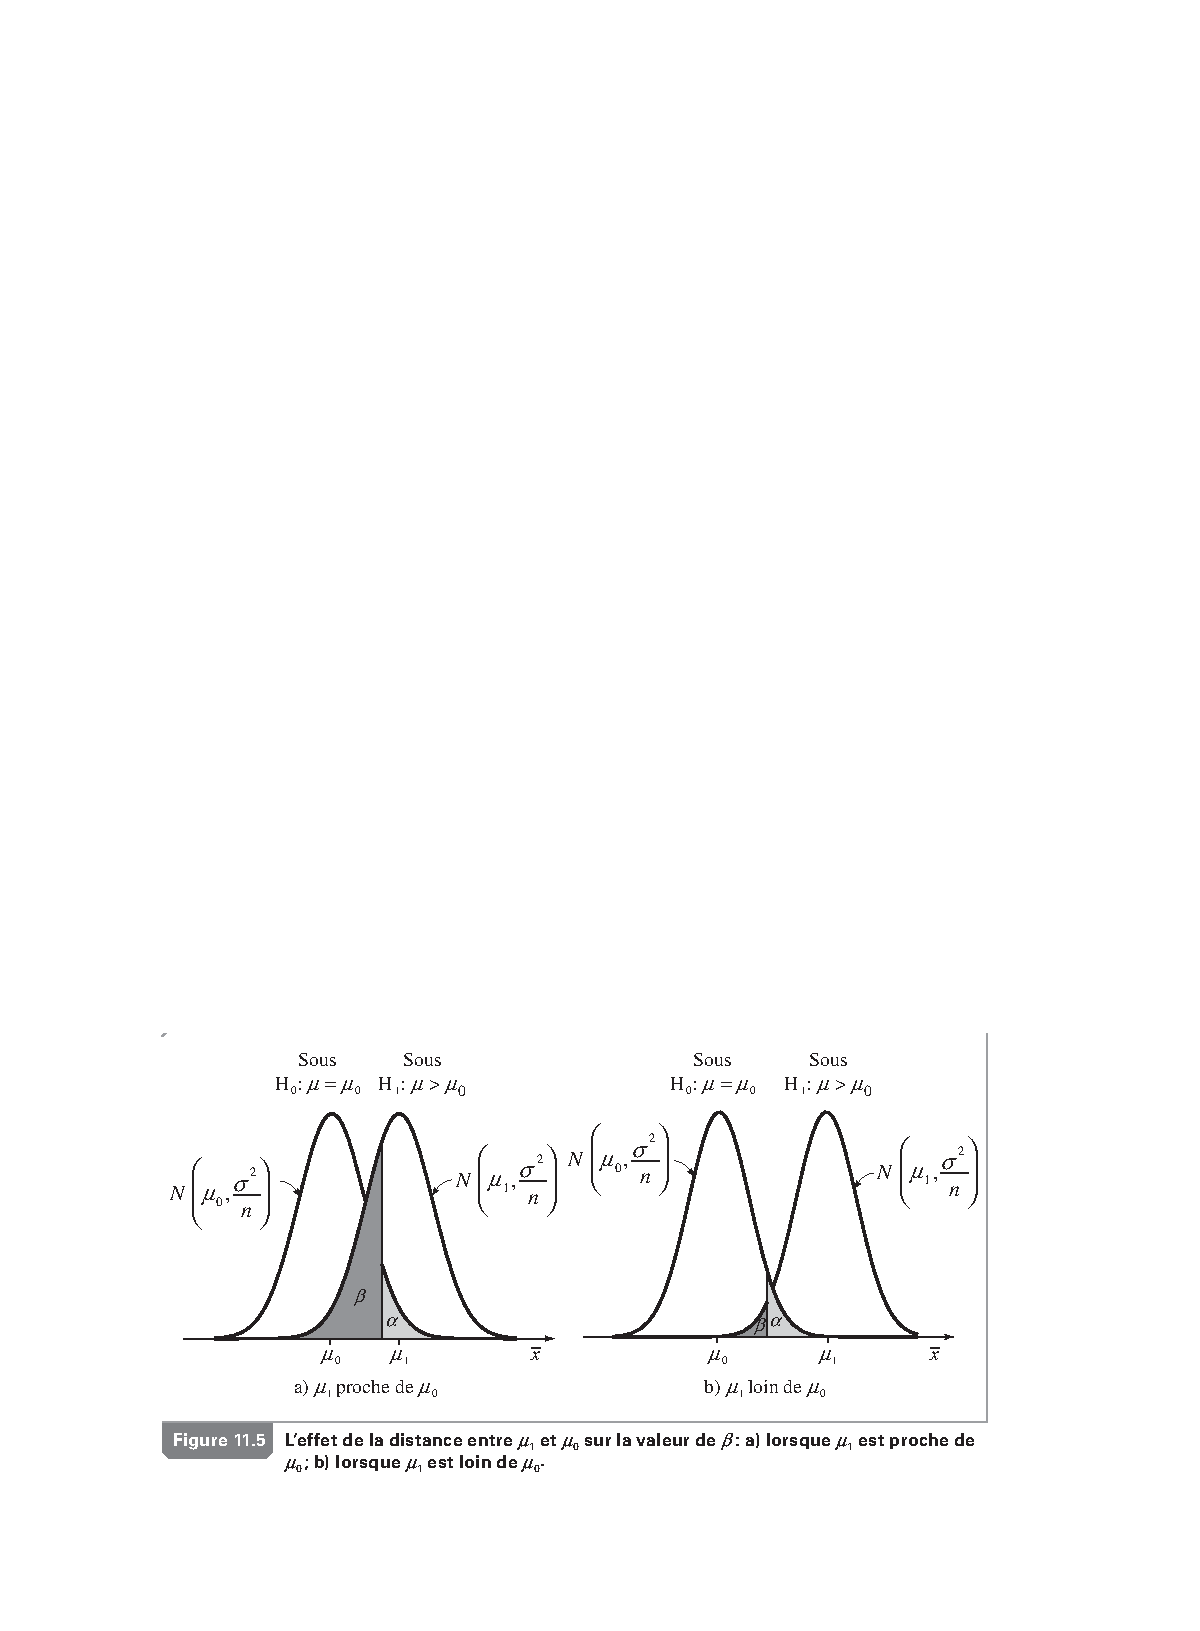
\includegraphics[width=0.88\textwidth, trim={0 36pt 4pt 6pt}, clip]{images/puiss1.pdf}

  \raggedright
  \medskip
  Plus la vraie valeur $\mu_1$ est \alert{éloignée} de $\mu_0$, plus $\beta$ est petit et plus la \alert{puissance est grande} : les grands effets sont plus faciles à détecter.
\end{frame}

\begin{frame}[t]{Déterminant 2 : la taille d'échantillon $n$}
  \centering
  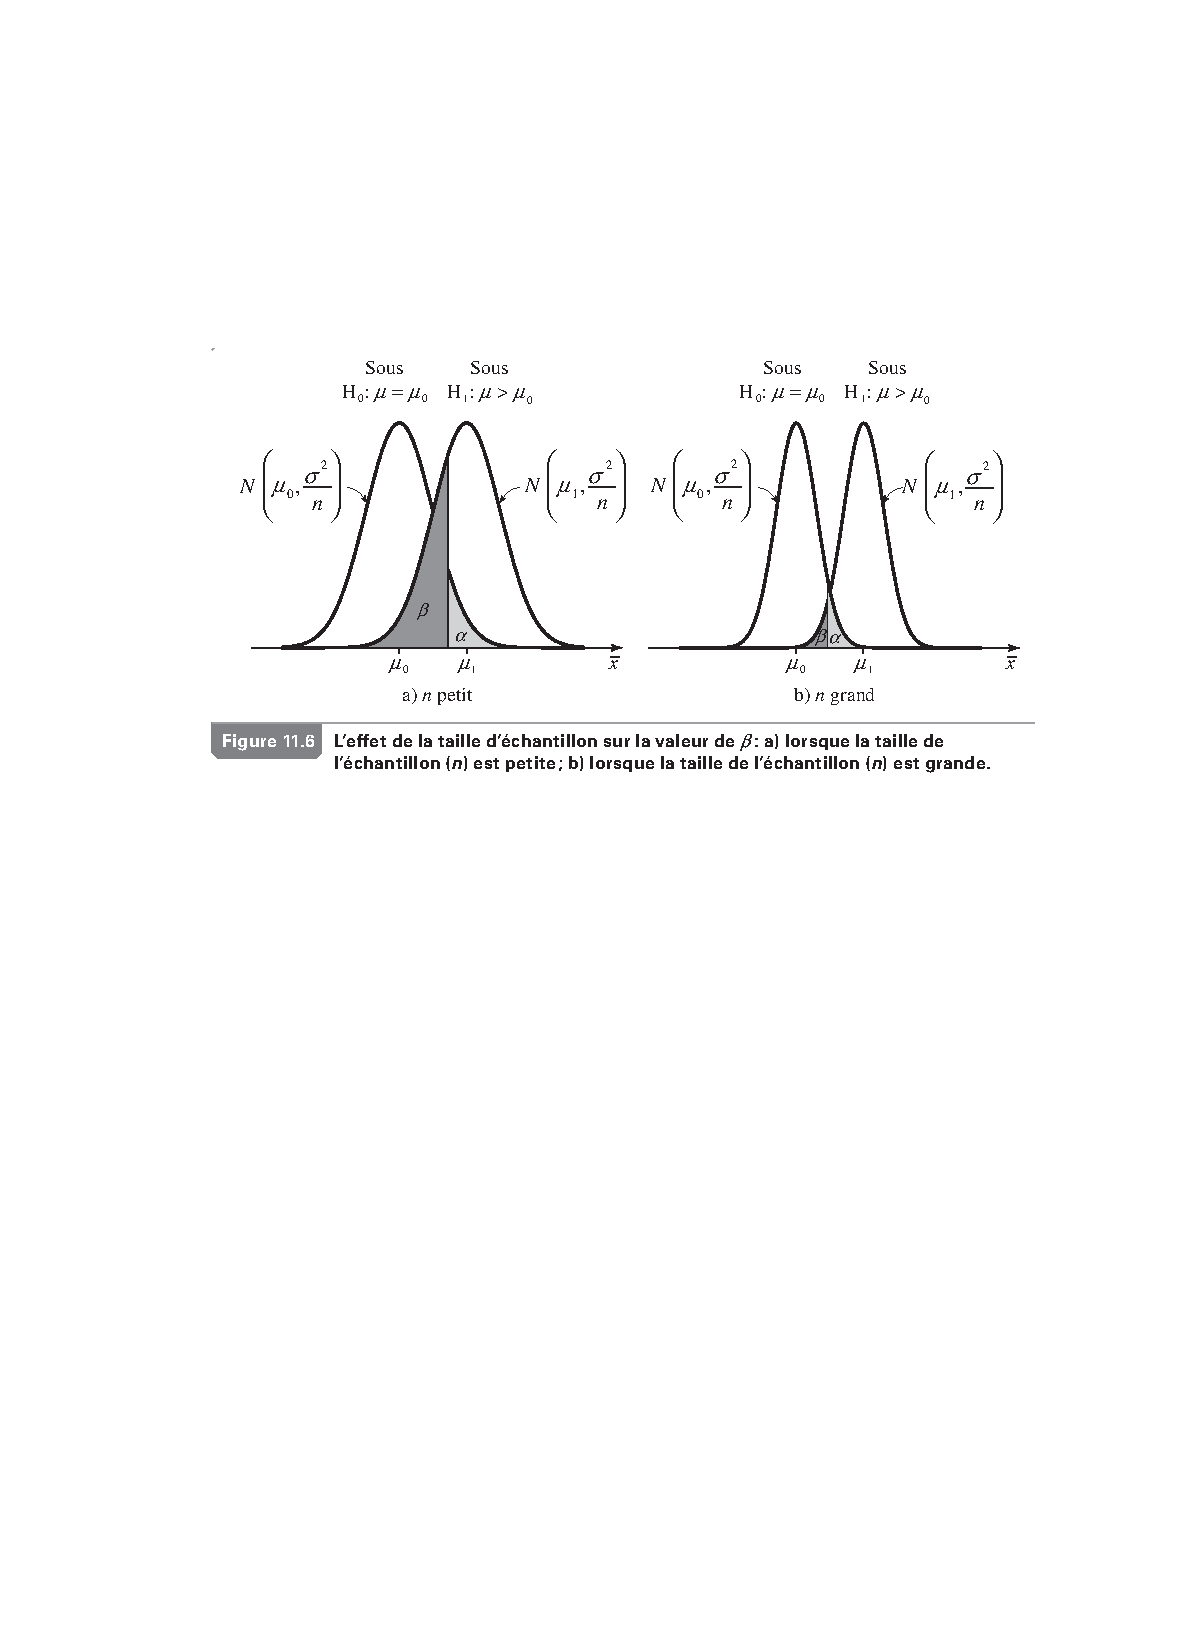
\includegraphics[width=0.88\textwidth, trim={0 40pt 4pt 6pt}, clip]{images/puiss2.pdf}

  \raggedright
  \medskip
  Quand $n$ augmente, les deux lois de $\overline{X}$ se \alert{resserrent} ($\sigma/\sqrt{n}$ diminue) : elles se chevauchent moins et la \alert{puissance augmente}.
\end{frame}

\begin{frame}[t]{Déterminant 3 : le seuil $\alpha$}
  \centering
  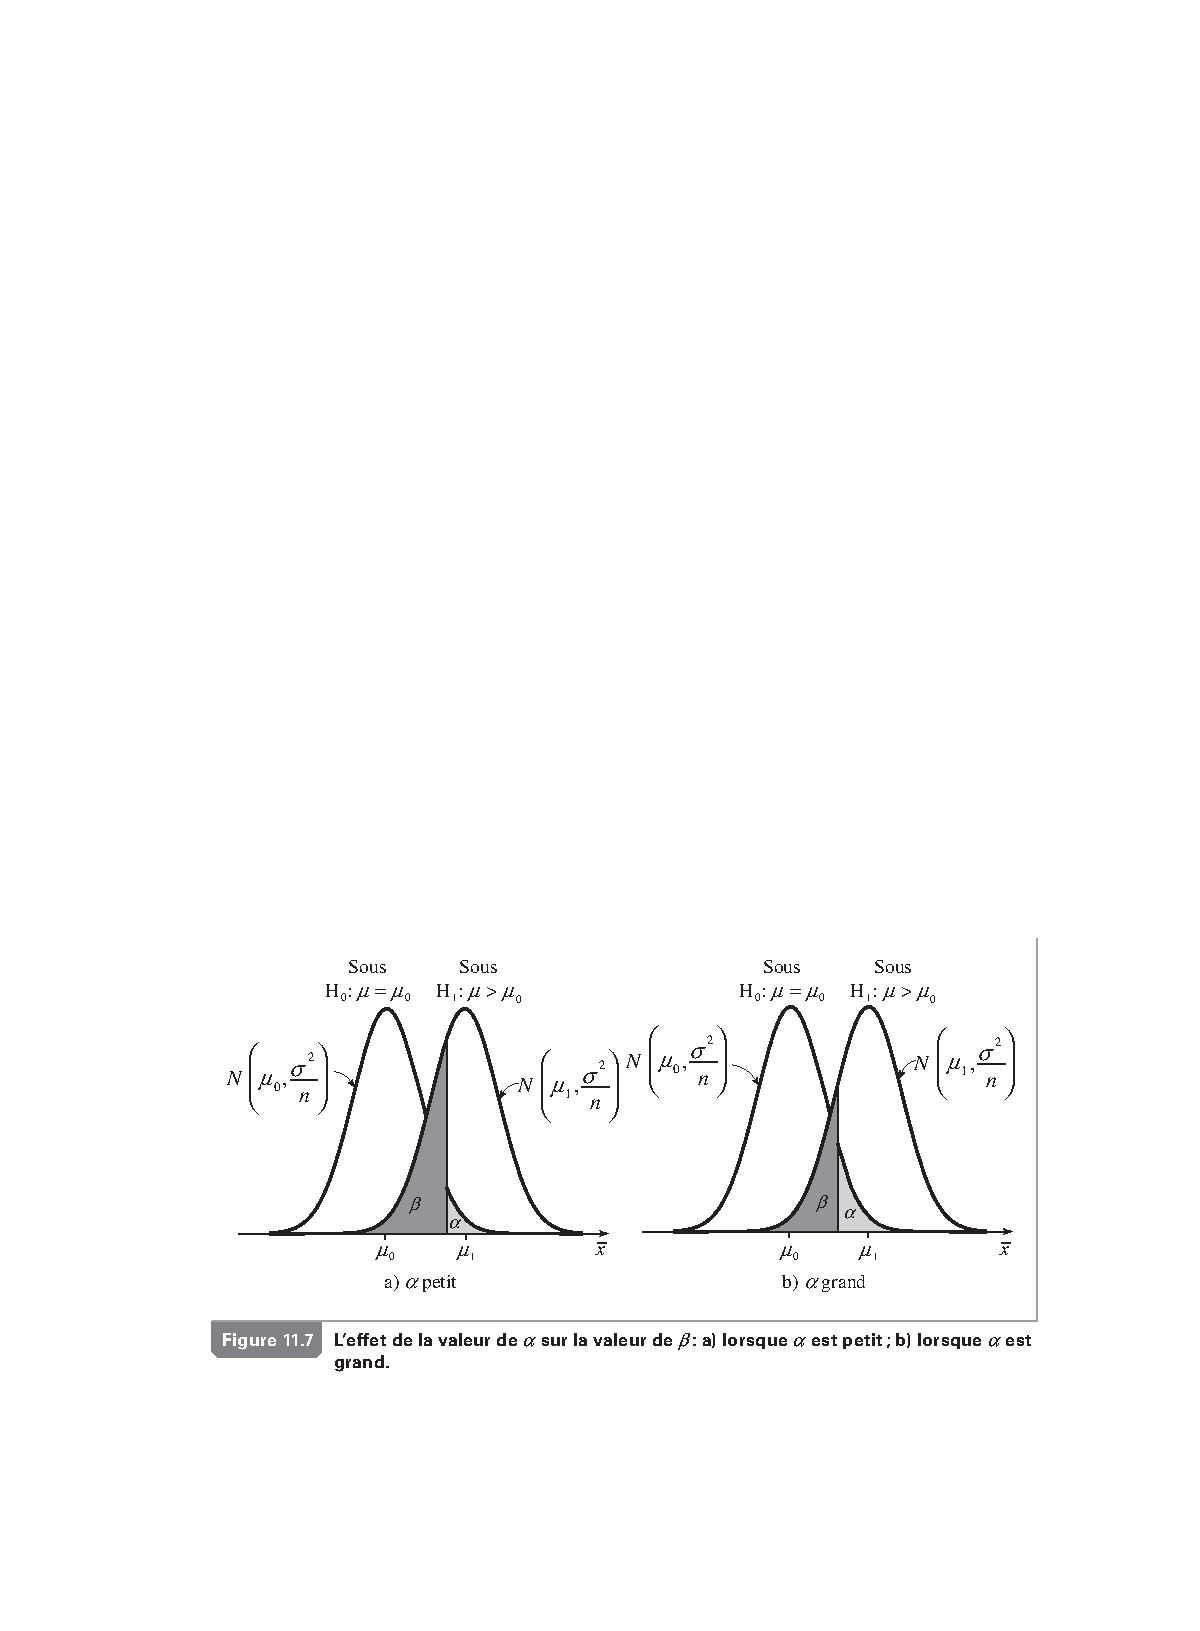
\includegraphics[width=0.88\textwidth, trim={0 48pt 4pt 6pt}, clip]{images/puiss3.pdf}

  \raggedright
  \medskip
  Un $\alpha$ plus grand déplace la frontière de rejet vers $\mu_0$ : la \alert{puissance augmente}, mais au prix de plus d'erreurs de type I.
\end{frame}

\begin{frame}[t]{En résumé : comment augmenter la puissance?}
  \textbf{Exemple 7} ($\mu_0 = 25$, $\mu_1 = 26$, $\sigma = 2$) :

  \medskip
  \centering
  \renewcommand{\arraystretch}{1.3}
  \begin{tabular}{ccc@{\hspace{1.5cm}}ccc}\toprule
    $\alpha$ & $n$ & \textbf{Puissance} & $\alpha$ & $n$ & \textbf{Puissance} \\ \midrule
    $0{,}01$ & 16 & $0{,}37$ & $0{,}05$ & 16 & $0{,}64$ \\
    $0{,}05$ & 16 & $0{,}64$ & $0{,}05$ & 25 & $0{,}80$ \\
    $0{,}10$ & 16 & $0{,}76$ & $0{,}05$ & 36 & $0{,}91$ \\ \bottomrule
  \end{tabular}

  \raggedright
  \medskip
  \begin{enumerate}\itemsep 1mm
    \item<2-> On ne contrôle pas $\mu_1$ : on demande au chercheur la \alert{plus petite différence importante} à détecter.
    \item<3-> Augmenter $\alpha$ est rarement acceptable (plus de faux positifs).
    \item<4-> En pratique, le levier principal est la \alert{taille d'échantillon} $n$, à planifier \alert{avant} l'étude.
  \end{enumerate}
\end{frame}

\begin{frame}[t]{Taille d'échantillon pour une puissance donnée}
  Pour un test unilatéral sur $\mu$ ($\sigma$ connue), seuil $\alpha$, puissance $1-\beta$ pour détecter un écart $\delta = |\mu_1 - \mu_0|$ :
  \begin{Boite}{Taille d'échantillon}
    $$n \ge \left(\frac{(z_{\alpha} + z_{\beta})\,\sigma}{\delta}\right)^2 \qquad \text{(bilatéral : remplacer } z_\alpha \text{ par } z_{\alpha/2})$$
  \end{Boite}

  \vspace{-1mm}
  \uncover<2->{
    \textbf{Exemple 7 :} combien de souris pour une puissance de 80\% si $\mu_1 = 26$?
    $$n \ge \left(\frac{(1{,}645 + 0{,}842) \times 2}{1}\right)^2 = 24{,}7 \quad\Longrightarrow\quad \mathbf{n = 25}\ \text{souris.}$$
  }

  \vspace{-2mm}
  \uncover<3->{
    \small Pour $\sigma$ inconnue, les calculs font intervenir une loi de Student « décentrée » ; R le fait avec \texttt{power.t.test()}.
  }
\end{frame}

\begin{frame}[plain,t]
  \centerline{\LARGE\bfseries\alert{QUIZ !}}

  \medskip
  Vrai ou faux?
  \begin{itemize}\itemsep 1.1cm
    \item Passer de $\alpha = 5\%$ à $\alpha = 1\%$ augmente la puissance du test.
    \item<2-> Il est plus facile de détecter une augmentation de 2\,g que de 0,5\,g.
    \item<3-> Avec seulement 5 souris par expérience, un résultat non significatif montre que la diète est inefficace.
    \item<4-> Un comité d'éthique animale peut exiger un calcul de puissance avant une expérience.
  \end{itemize}
\end{frame}

%===============================================================================
\section{Tests sur une moyenne \texorpdfstring{$\mu$}{mu}}
%===============================================================================

\begin{frame}[t]{Test $t$ sur $\mu$ : loi normale, $\sigma$ inconnue}
  En pratique, $\sigma$ est inconnue : on la remplace par $S$ (comme pour l'IC du chapitre 3b).
  \begin{Boite}{Statistique de test}
    \vspace{-2mm}
    $$T_0 = \frac{\overline{X} - \mu_0}{S/\sqrt{n}} \sim t_{n-1} \quad \text{sous } H_0 : \mu = \mu_0 \qquad \text{valeur observée : } t_{obs}$$
  \end{Boite}

  \vspace{-3mm}
  \centering
  \renewcommand{\arraystretch}{1.3}
  \small
  \begin{tabular}{lll}\toprule
    \textbf{Alternative} & \textbf{Rejeter $H_0$ si} & \textbf{Valeur-p} \\ \midrule
    $H_1 : \mu \ne \mu_0$ & $|t_{obs}| > t_{n-1,\,\alpha/2}$ & $2\,P(t_{n-1} \ge |t_{obs}|)$ \\
    $H_1 : \mu > \mu_0$ & $t_{obs} > t_{n-1,\,\alpha}$ & $P(t_{n-1} \ge t_{obs})$ \\
    $H_1 : \mu < \mu_0$ & $t_{obs} < -t_{n-1,\,\alpha}$ & $P(t_{n-1} \le t_{obs})$ \\ \bottomrule
  \end{tabular}

  \raggedright
  \smallskip
  Ce sont les mêmes règles qu'au chapitre 4, avec d'autres degrés de liberté.
\end{frame}

\begin{frame}[t]{Exemple 1 (retour) : la pression artérielle}
  Mesures ($n = 7$) : 141, 130, 135, 138, 137, 122, 135 ; $\bar{x} = 134$, $s = 6{,}27$\,mm\,Hg.
  Une étude affirme que la pression systolique moyenne de cette population est de 130\,mm\,Hg. Nos données contredisent-elles cette valeur ($\alpha = 5\%$)?

  \medskip
  \begin{enumerate}\itemsep 1.5mm
    \item<2-> \textbf{Hypothèses :} $H_0 : \mu = 130$ contre $H_1 : \mu \ne 130$ (bilatéral).
    \item<3-> \textbf{Règle :} rejeter $H_0$ si $|t_{obs}| > t_{6,\,0{,}025} = 2{,}447$.
    \item<4-> \textbf{Calcul :} $t_{obs} = \dfrac{134 - 130}{6{,}27/\sqrt{7}} = \dfrac{4}{2{,}37} = \mathbf{1{,}69}$.
    \item<5-> \textbf{Décision :} $|1{,}69| < 2{,}447$ : on \alert{ne rejette pas} $H_0$ (valeur-p $= 0{,}14$).
    \item<6-> \textbf{Conclusion :} au seuil de 5\%, les données ne permettent pas de conclure que la pression moyenne diffère de 130\,mm\,Hg.
  \end{enumerate}
\end{frame}

\begin{frame}[t]{Exemple 1 (retour) : la valeur-p en image}
  \centering
  \begin{tikzpicture}
    \begin{axis}[cloche, width=11cm, height=4.6cm, xmin=-4.5, xmax=4.5, ymax=0.42,
      xtick={-2.447,-1.687,0,1.687,2.447}, xticklabels={$-2{,}447$, $-1{,}69$, 0, $1{,}69$, $2{,}447$},
      title={Loi $t_6$ (loi de $T_0$ si $H_0$ est vraie)}]
      \addplot[draw=none, fill=Accent!70, domain=-4.5:-1.687, samples=40] {\dtsix} \closedcycle;
      \addplot[draw=none, fill=Accent!70, domain=1.687:4.5, samples=40] {\dtsix} \closedcycle;
      \addplot[draw=none, fill=rougelaval!60, domain=-4.5:-2.447, samples=30] {\dtsix} \closedcycle;
      \addplot[draw=none, fill=rougelaval!60, domain=2.447:4.5, samples=30] {\dtsix} \closedcycle;
      \addplot[thick, Dominante!70!black, domain=-4.5:4.5, samples=120] {\dtsix};
      \node[font=\scriptsize, Accent!80!black] at (axis cs:3.2,0.2) {$0{,}071$};
      \draw[->, Accent!80!black] (axis cs:3.2,0.18) -- (axis cs:2.0,0.05);
      \node[font=\scriptsize, Accent!80!black] at (axis cs:-3.2,0.2) {$0{,}071$};
      \draw[->, Accent!80!black] (axis cs:-3.2,0.18) -- (axis cs:-2.0,0.05);
    \end{axis}
  \end{tikzpicture}

  \raggedright
  \small
  \begin{itemize}\itemsep 1mm
    \item Valeur-p $= P(|t_6| \ge 1{,}69) = 2 \times 0{,}071 = \mathbf{0{,}14}$ (aire orange totale) $> 0{,}05$.
    \item Région de rejet au seuil de 5\% (en rouge) : $|t| > 2{,}447$ ; $t_{obs} = 1{,}69$ n'y tombe pas.
  \end{itemize}
\end{frame}

\begin{frame}[fragile,t]{Exemple 1 (retour) : avec R}
  \footnotesize
\begin{verbatim}
> x <- c(141, 130, 135, 138, 137, 122, 135)
> t.test(x, mu = 130)

        One Sample t-test

data:  x
t = 1.6874, df = 6, p-value = 0.1425
alternative hypothesis: true mean is not equal to 130
95 percent confidence interval:
 128.1997 139.8003
sample estimates:
mean of x
      134
\end{verbatim}

  \small
  Options : \texttt{alternative = "greater"} ($H_1 : \mu > \mu_0$) ou \texttt{"less"} ; \texttt{conf.level = 0.99}.
  Sans \texttt{mu = }, R teste $H_0 : \mu = 0$ (rarement pertinent !).
\end{frame}

\begin{frame}[t]{Ne pas rejeter $H_0$ ne veut pas dire $\mu = 130$ !}
  \begin{itemize}\itemsep 4mm
    \item Avec seulement $n = 7$ personnes, l'erreur-type ($2{,}37$) est grande : le test a \alert{peu de puissance}.
    \item<2-> L'IC à 95\% $[128{,}20 \,;\, 139{,}80]$ contient 130, mais aussi 135 ou 139 : beaucoup de valeurs de $\mu$ restent \alert{plausibles}.
    \item<3-> Conclusion correcte : « les données sont \alert{compatibles} avec $\mu = 130$ », et non « on a montré que $\mu = 130$ ».
  \end{itemize}

  \bigskip
  \uncover<4->{
  \begin{Boite}{Bonne pratique}
    Rapporter à la fois la \alert{valeur-p} et l'\alert{intervalle de confiance} : l'IC montre l'ampleur plausible de l'effet et la précision obtenue.
  \end{Boite}
  }
\end{frame}

\begin{frame}[t]{Cas $n$ grand, loi inconnue : exemple 3 (mercure)}
  Si $n$ est grand ($n \ge 30$), par le TLC :
  $\;Z_0 = \dfrac{\overline{X} - \mu_0}{S/\sqrt{n}} \approx \mathcal{N}(0,1)$ sous $H_0$ (niveau approximatif).

  \medskip
  \textbf{Exemple 3 :} $n = 50$ dorés, $\bar{x} = 0{,}42\ \mu$g/g, $s = 0{,}18\ \mu$g/g. La concentration moyenne est-elle \alert{inférieure} à la ligne directrice de $0{,}5\ \mu$g/g ($\alpha = 1\%$)?

  \medskip
  \begin{enumerate}\itemsep 1.5mm
    \item<2-> $H_0 : \mu = 0{,}5$ contre $H_1 : \mu < 0{,}5$.
    \item<3-> Rejeter $H_0$ si $z_{obs} < -z_{0{,}01} = -2{,}326$.
    \item<4-> $z_{obs} = \dfrac{0{,}42 - 0{,}5}{0{,}18/\sqrt{50}} = \dfrac{-0{,}08}{0{,}0255} = \mathbf{-3{,}14}$.
    \item<5-> $-3{,}14 < -2{,}326$ : on \alert{rejette $H_0$} (valeur-p $= P(Z \le -3{,}14) = 0{,}0008$).
    \item<6-> Au seuil de 1\%, la concentration moyenne est significativement inférieure à $0{,}5\ \mu$g/g.
  \end{enumerate}
\end{frame}

\begin{frame}[t]{Exemple 9 : nitrates dans l'eau de puits}
  On mesure la concentration d'azote des nitrates (mg/L) dans 12 puits d'une zone agricole. La norme de qualité de l'eau potable est de \alert{10\,mg/L}.

  \medskip
  \centering
  9,8 \quad 12,4 \quad 10,9 \quad 13,1 \quad 8,7 \quad 11,5 \quad 12,8 \quad 10,2 \quad 9,5 \quad 13,6 \quad 11,9 \quad 10,6

  \raggedright
  \medskip
  On suppose les concentrations normales. $\bar{x} = 11{,}25$\,mg/L et $s = 1{,}55$\,mg/L.

  \medskip
  \begin{enumerate}\itemsep 2.5mm
    \item Au seuil de 5\%, la concentration moyenne \alert{dépasse}-t-elle la norme? Suivez les 5 étapes.
    \item Donnez un encadrement de la valeur-p à l'aide de la table de Student, puis la commande R qui la calcule.
    \item Pourquoi un test unilatéral est-il justifié ici?
  \end{enumerate}

  \medskip
  \small (Réponses à la fin du chapitre.)
\end{frame}

%===============================================================================
\section{Tests sur une proportion et sur une variance}
%===============================================================================

\begin{frame}[t]{Test sur une proportion}
  $Y \sim \text{Binomiale}(n, p)$, $\hat{p} = y/n$. On teste $H_0 : p = p_0$.

  \begin{Boite}{Statistique de test (approximation normale)}
    $$Z_0 = \frac{\widehat{P} - p_0}{\sqrt{p_0(1-p_0)/n}} \approx \mathcal{N}(0,1) \quad \text{sous } H_0,
    \qquad \text{si } np_0 \ge 5 \text{ et } n(1-p_0) \ge 5.$$
  \end{Boite}

  \vspace{-3mm}
  \begin{itemize}\itemsep 1mm
    \item<2-> Mêmes règles de décision et valeurs-p que pour $Z_0$ sur $\mu$ (unilatéral ou bilatéral).
    \item<3-> \alert{Attention :} l'erreur-type utilise $p_0$ (la valeur supposée sous $H_0$), alors que l'IC du chapitre 3b utilise $\hat{p}$.
    \item<4-> Si $n$ est petit, on utilise le \alert{test binomial exact} (\texttt{binom.test()} dans R), qui calcule la valeur-p directement avec la loi binomiale.
  \end{itemize}
\end{frame}

\begin{frame}[t]{Exemple 4 (retour) : infection chez des veaux}
  Sur 80 veaux, 12 sont infectés ($\hat{p} = 0{,}15$). Le vétérinaire intervient si la prévalence \alert{dépasse 10\%}. Au seuil de 5\%?

  \medskip
  \begin{enumerate}\itemsep 1.5mm
    \item<2-> $H_0 : p = 0{,}10$ contre $H_1 : p > 0{,}10$. Conditions : $80 \times 0{,}10 = 8 \ge 5$ et $72 \ge 5$.
    \item<3-> Rejeter $H_0$ si $z_{obs} > z_{0{,}05} = 1{,}645$.
    \item<4-> $z_{obs} = \dfrac{0{,}15 - 0{,}10}{\sqrt{0{,}10 \times 0{,}90 / 80}} = \dfrac{0{,}05}{0{,}0335} = \mathbf{1{,}49}$.
    \item<5-> $1{,}49 < 1{,}645$ : on \alert{ne rejette pas $H_0$} (valeur-p $= P(Z \ge 1{,}49) = 0{,}068$).
    \item<6-> Au seuil de 5\%, les données ne démontrent pas que la prévalence dépasse 10\%.
  \end{enumerate}

  \medskip
  \uncover<7->{
    \small Remarque : $\hat{p} = 15\%$ est pourtant supérieur à 10\%\ldots\ mais avec 80 veaux, un tel écart peut facilement survenir par hasard.
  }
\end{frame}

\begin{frame}[fragile,t]{Exemple 4 (retour) : avec R}
  \footnotesize
\begin{verbatim}
> prop.test(12, 80, p = 0.10, alternative = "greater",
+           correct = FALSE)
X-squared = 2.2222, df = 1, p-value = 0.06802
> binom.test(12, 80, p = 0.10, alternative = "greater")
number of successes = 12, number of trials = 80,
p-value = 0.1004
\end{verbatim}

  \small
  \begin{itemize}\itemsep 2mm
    \item \texttt{prop.test(..., correct = FALSE)} reproduit le calcul à la main ($z_{obs}^2 = 1{,}49^2 = 2{,}22$).
    \item \texttt{binom.test()} donne la valeur-p \alert{exacte} : $P(Y \ge 12 \mid n = 80,\ p = 0{,}10) = 0{,}100$.
    \item Avec $np_0 = 8$, l'approximation normale est grossière : on préfère le test exact. La conclusion est la même.
  \end{itemize}
\end{frame}

\begin{frame}[plain,t]
  \centerline{\LARGE\bfseries\alert{QUIZ !}}

  \medskip
  Exemple 2 (sondage) : sur $n = 1028$ Québécois, 216 citent l'environnement ($\hat{p} = 0{,}2101$). Un groupe affirme que \alert{25\%} des Québécois ont cette opinion.
  \begin{itemize}\itemsep 1.1cm
    \item Formulez $H_0$ et $H_1$ pour vérifier cette affirmation.
    \item<2-> Calculez $z_{obs}$ et la valeur-p. Conclusion au seuil de 5\%?
    \item<3-> Retrouvez la conclusion à l'aide de l'IC à 95\% du chapitre 3b : $[0{,}185 \,;\, 0{,}235]$.
  \end{itemize}
\end{frame}

\begin{frame}[t]{Test sur $\sigma^2$ : population normale}
  Pour contrôler la \alert{variabilité} (uniformité d'un produit, précision d'un appareil), on teste $H_0 : \sigma^2 = \sigma_0^2$.

  \begin{Boite}{Statistique de test}
    \vspace{-2mm}
    $$U_0 = \frac{(n-1)S^2}{\sigma_0^2} \sim \chi^2_{n-1} \quad \text{sous } H_0 \qquad \text{valeur observée : } u_{obs}$$
  \end{Boite}

  \vspace{-3mm}
  \centering
  \renewcommand{\arraystretch}{1.3}
  \small
  \begin{tabular}{lll}\toprule
    \textbf{Alternative} & \textbf{Rejeter $H_0$ si} & \textbf{Valeur-p} \\ \midrule
    $H_1 : \sigma^2 > \sigma_0^2$ & $u_{obs} > \chi^2_{n-1,\,\alpha}$ & $P(\chi^2_{n-1} \ge u_{obs})$ \\
    $H_1 : \sigma^2 < \sigma_0^2$ & $u_{obs} < \chi^2_{n-1,\,1-\alpha}$ & $P(\chi^2_{n-1} \le u_{obs})$ \\
    $H_1 : \sigma^2 \ne \sigma_0^2$ & $u_{obs} < \chi^2_{n-1,\,1-\alpha/2}$ ou $u_{obs} > \chi^2_{n-1,\,\alpha/2}$ & $2 \times$ la plus petite queue \\ \bottomrule
  \end{tabular}

  \raggedright
  \small Comme pour l'IC, ce test est \alert{très sensible à la normalité}.
\end{frame}

\begin{frame}[t]{Exemple 10 : uniformité de comprimés}
  Un fabricant exige que l'écart-type de la quantité de principe actif par comprimé ne dépasse pas \alert{2\,mg} ($\sigma_0^2 = 4$\,mg$^2$). Sur $n = 20$ comprimés d'un nouveau lot, $s = 2{,}6$\,mg. La variabilité est-elle trop grande ($\alpha = 5\%$)?

  \medskip
  \begin{enumerate}\itemsep 1.5mm
    \item<2-> $H_0 : \sigma^2 = 4$ contre $H_1 : \sigma^2 > 4$.
    \item<3-> Rejeter $H_0$ si $u_{obs} > \chi^2_{19;\,0{,}05} = 30{,}144$.
    \item<4-> $u_{obs} = \dfrac{19 \times 2{,}6^2}{4} = \dfrac{19 \times 6{,}76}{4} = \mathbf{32{,}11}$.
    \item<5-> $32{,}11 > 30{,}144$ : on \alert{rejette $H_0$} (valeur-p $= P(\chi^2_{19} \ge 32{,}11) = 0{,}030$).
    \item<6-> Au seuil de 5\%, l'écart-type du lot dépasse significativement 2\,mg : le lot ne respecte pas l'exigence d'uniformité.
  \end{enumerate}

  \medskip
  \uncover<5->{
    \small Dans R : \texttt{u <- 19 * 2.6\textasciicircum 2 / 4 ; 1 - pchisq(u, df = 19)}.
  }
\end{frame}

%===============================================================================
\section{Bien interpréter un test : IC et importance pratique}
%===============================================================================

\begin{frame}[t]{IC et test bilatéral : deux faces d'une même médaille}
  \begin{Boite}{Équivalence}
    On rejette $H_0 : \theta = \theta_0$ contre $H_1 : \theta \ne \theta_0$ au seuil $\alpha$
    $\iff$ l'IC de niveau $1-\alpha$ pour $\theta$ \alert{ne contient pas} $\theta_0$.
  \end{Boite}

  \vspace{-1mm}
  \uncover<2->{
    \textbf{Pourquoi?} Pour $\mu$ : $|t_{obs}| \le t_{n-1,\,\alpha/2} \iff |\bar{x} - \mu_0| \le t_{n-1,\,\alpha/2}\,\frac{s}{\sqrt{n}} \iff \mu_0 \in \bar{x} \pm \text{ME}$.
  }

  \medskip
  \uncover<3->{
  \textbf{Exemples :}
  \begin{itemize}\itemsep 1.5mm
    \item Pression : l'IC à 95\% $[128{,}20 \,;\, 139{,}80]$ contient 130 $\Rightarrow$ on ne rejette pas $H_0 : \mu = 130$ (valeur-p $= 0{,}14$).
    \item Mercure : l'IC à 95\% $[0{,}370 \,;\, 0{,}470]$ exclut $0{,}5$ $\Rightarrow$ on rejette $H_0 : \mu = 0{,}5$ en bilatéral à 5\%.
  \end{itemize}
  }

  \uncover<4->{
    \small L'IC donne \alert{plus d'information} : il indique toutes les valeurs de $\theta_0$ qu'on ne rejetterait pas. Cette équivalence vaut aussi pour $\sigma^2$ (et, approximativement, pour $p$).
  }
\end{frame}

\begin{frame}[plain,t]
  \centerline{\LARGE\bfseries\alert{QUIZ !}}

  \medskip
  Dans un lac, l'IC à 99\% pour la concentration moyenne de chlorophylle $a$ est $[2{,}26 \,;\, 3{,}41]\ \mu$g/L. Tests bilatéraux : vrai, faux ou information insuffisante?
  \begin{itemize}\itemsep 1.0cm
    \item Au seuil de 1\%, on rejette $H_0 : \mu = 3$.
    \item<2-> Au seuil de 1\%, on rejette $H_0 : \mu = 4$.
    \item<3-> Au seuil de 5\%, on rejette $H_0 : \mu = 4$.
    \item<4-> Au seuil de 5\%, on rejette $H_0 : \mu = 2{,}5$.
  \end{itemize}
\end{frame}

\begin{frame}[t]{« Statistiquement significatif » $\ne$ « important »}
  Une étude sur $n = 5000$ adultes mesure l'effet d'une diète sur la pression systolique : baisse moyenne de $\bar{d} = 0{,}8$\,mm\,Hg, $s = 12$\,mm\,Hg.

  \uncover<2->{
    $H_0 : \mu_D = 0$ : $\;t_{obs} = \dfrac{0{,}8}{12/\sqrt{5000}} = 4{,}71$, \ valeur-p $= 2{,}5 \times 10^{-6}$. \ \alert{Très significatif !}
  }

  \uncover<3->{
    Mais l'IC à 95\% pour la baisse moyenne est $[0{,}47 \,;\, 1{,}13]$\,mm\,Hg : un effet \alert{cliniquement négligeable}.
  }

  \vspace{-2mm}
  \uncover<4->{
  \begin{Boite}{À retenir}
    \small
    \begin{itemize}\itemsep 0mm
      \item Avec un très grand $n$, presque toute différence devient significative.
      \item Avec un petit $n$, un effet important peut ne pas être significatif (faible puissance).
      \item L'importance pratique se juge avec l'\alert{estimation} et son \alert{IC}, selon l'expertise du domaine.
    \end{itemize}
  \end{Boite}
  }
\end{frame}

\begin{frame}[plain,t]
  \centerline{\LARGE\bfseries\alert{QUIZ !}}

  \medskip
  Vrai ou faux?
  \begin{itemize}\itemsep 1.2cm
    \item Une valeur-p de $0{,}0001$ indique que l'effet du traitement est très grand.
    \item<2-> Deux études testent le même traitement. L'étude A ($n = 20$) donne $p = 0{,}20$ et l'étude B ($n = 2000$) donne $p = 0{,}001$. L'étude B a nécessairement trouvé un effet plus grand.
    \item<3-> Pour juger de l'importance d'un effet, on doit regarder l'estimation et son intervalle de confiance.
  \end{itemize}
\end{frame}

%===============================================================================
\section{Synthèse}
%===============================================================================

\begin{frame}[t]{Tableau récapitulatif : tests à un échantillon}
  \centering
  \footnotesize
  \renewcommand{\arraystretch}{1.7}
  \begin{tabular}{llll}\toprule
    \textbf{Hypothèse nulle} & \textbf{Statistique} & \textbf{Loi sous $H_0$} & \textbf{R} \\ \midrule
    $\mu = \mu_0$ (normale, $\sigma$ connue) & $z_{obs} = \frac{\bar{x} - \mu_0}{\sigma/\sqrt{n}}$ & $\mathcal{N}(0,1)$ & \texttt{pnorm()} \\
    $\mu = \mu_0$ (normale, $\sigma$ inconnue) & $t_{obs} = \frac{\bar{x} - \mu_0}{s/\sqrt{n}}$ & $t_{n-1}$ & \texttt{t.test(x, mu = )} \\
    $\mu = \mu_0$ ($n$ grand) & $z_{obs} = \frac{\bar{x} - \mu_0}{s/\sqrt{n}}$ & $\approx \mathcal{N}(0,1)$ & \texttt{t.test(x, mu = )} \\
    $p = p_0$ ($np_0,\ n(1-p_0) \ge 5$) & $z_{obs} = \frac{\hat{p} - p_0}{\sqrt{p_0(1-p_0)/n}}$ & $\approx \mathcal{N}(0,1)$ & \texttt{prop.test()} \\
    $\sigma^2 = \sigma_0^2$ (normale) & $u_{obs} = \frac{(n-1)s^2}{\sigma_0^2}$ & $\chi^2_{n-1}$ & \texttt{pchisq()} \\ \bottomrule
  \end{tabular}

  \raggedright
  \medskip
  \normalsize
  Dans tous les cas : \alert{rejeter $H_0$ si valeur-p $\le \alpha$}. Au \alert{chapitre 4}, on applique la même démarche pour \alert{comparer deux populations}.
\end{frame}

\begin{frame}[t]{Réponses aux exemples}
  \footnotesize
  \begin{itemize}\itemsep 1mm
    \item \textbf{Quiz ($H_0$/$H_1$) :} $H_0 : \mu = 3{,}5$ vs $H_1 : \mu > 3{,}5$ ; \ $H_0 : p = 0{,}20$ vs $H_1 : p > 0{,}20$ ; \ $H_0 : \mu = 72$ vs $H_1 : \mu \ne 72$. Avec $\bar{x} = 3{,}62$ seulement, on ne peut rien conclure : il faut connaître la variabilité (erreur-type) pour juger si l'écart de $0{,}12$ dépasse le hasard.
    \item \textbf{Exemple 7 :} $z_{obs} = 2{,}2 > 1{,}645$, rejet de $H_0$ ; valeur-p $= 0{,}0139$ ; puissance à $\mu_1 = 26$ : $0{,}639$ ; $n = 25$ pour 80\%.
    \item \textbf{Quiz (erreurs) :} type I : conclure que la diète augmente la masse alors qu'elle ne le fait pas ; type II : ne pas détecter une augmentation réelle. Pour une maladie grave, le faux négatif (type II) est le plus grave : on privilégie la puissance (sensibilité). Faux : $1-\alpha$ n'est pas $P(H_0 \text{ vraie})$.
    \item \textbf{Quiz (valeur-p, plantules) :} V ; F ; V ; F (avec $\mu_0 = 4$, la valeur-p est plus grande que $0{,}09$) ; info insuffisante ; F (erreur-type plus petite, donc valeur-p plus petite).
    \item \textbf{Quiz (unilatéral) :} V ; V ; F ($0{,}08 > 0{,}05$).
    \item \textbf{Quiz (puissance) :} F ; V ; F (puissance très faible) ; V.
  \end{itemize}
\end{frame}

\begin{frame}[t]{Réponses aux exemples (suite)}
  \footnotesize
  \begin{itemize}\itemsep 1.5mm
    \item \textbf{Exemple 9 (nitrates) :} $H_0 : \mu = 10$ vs $H_1 : \mu > 10$ ; rejet si $t_{obs} > t_{11;\,0{,}05} = 1{,}796$ ; $t_{obs} = (11{,}25 - 10)/(1{,}551/\sqrt{12}) = 2{,}79$ : rejet de $H_0$. Valeur-p entre $0{,}005$ et $0{,}01$ ($t_{11;\,0{,}01} = 2{,}718$, $t_{11;\,0{,}005} = 3{,}106$) ; exacte : $0{,}0088$ avec \texttt{t.test(x, mu = 10, alternative = "greater")}. Unilatéral : seul un dépassement de la norme pose problème.
    \item \textbf{Exemple 4 (veaux) :} $z_{obs} = 1{,}49$, valeur-p $= 0{,}068$ (exacte : $0{,}100$) ; non-rejet.
    \item \textbf{Quiz (sondage) :} $H_0 : p = 0{,}25$ vs $H_1 : p \ne 0{,}25$ ; $z_{obs} = (0{,}2101 - 0{,}25)/\sqrt{0{,}25 \times 0{,}75/1028} = -2{,}95$ ; valeur-p $= 0{,}003$ : rejet. L'IC $[0{,}185 \,;\, 0{,}235]$ exclut $0{,}25$ : même conclusion.
    \item \textbf{Exemple 10 (comprimés) :} $u_{obs} = 32{,}11 > 30{,}144$ ; valeur-p $= 0{,}030$ : rejet.
    \item \textbf{Quiz (IC et test) :} F ; V ; V (l'IC à 95\% est inclus dans celui à 99\%) ; info insuffisante (l'IC à 95\% est plus étroit, mais on ne sait pas de combien).
    \item \textbf{Quiz (importance pratique) :} F ; F (la valeur-p dépend aussi de $n$) ; V.
  \end{itemize}
\end{frame}

\end{document}
